\documentclass{lmcs}
\pdfoutput=1

\usepackage{silence}
\WarningFilter{caption}{Unsupported document class}
\WarningFilter{remreset}{The remreset package is obsolete}

\usepackage{lastpage}
\lmcsdoi{15}{3}{16}
\lmcsheading{}{\pageref{LastPage}}{}{}{May~16,~2018}{Aug.~13,~2019}{}


\keywords{weighted automata,
Markov chains,
nested weighted automata,
expected value,
distribution}

\usepackage{amsmath,amsthm}

\newcommand{\Sskip}{\smallskip}
\newcommand{\proofideas}{\smallskip\noindent{\emph{The key ideas.}}}


\usepackage{amsthm}
\usepackage{amsfonts,graphicx,url,stfloats,subfig}
\usepackage{amssymb,amsmath,color,verbatim,bm}
\usepackage{stmaryrd,multirow}
\usepackage{environ,xspace}
\usepackage{thmtools,thm-restate,wrapfig}
\usepackage{tikz}
\usetikzlibrary{arrows,automata,shapes}

\usetikzlibrary{calc}

\newcommand{\Paragraph}[1]{\noindent{\textbf{#1}}}

\newcommand{\masterA}{\mathcal{A}_{\textrm{mas}}}
\newcommand{\nestedA}{\mathbb{A}}
\newcommand{\slaveA}{{\mathfrak{B}}}
\newcommand{\nonnestedA}{\mathcal{A}}
\newcommand{\selectA}{\mathcal{S}}

\newcommand{\masterStates}{Q_{\textrm{mas}}}

\newcommand{\finValFunc}{\textrm{FinValFunc}}


\newcommand{\silent}[1]{\mathsf{sil}({#1})} 

\newcommand{\cost}{{C}}

\newcommand{\masterRun}{\Pi}
\newcommand{\slaveRun}{\pi}
\newcommand{\lang}{\mathcal{L}}

\newcommand{\valueL}[1]{\mathcal{L}_{{#1}}}

\newcommand{\abs}{\mathop{\mathsf{Abs}}}

\newcommand{\EXPTIME}{\textsc{ExpTime}{}}
\newcommand{\PTIME}{\textsc{PTime}{}}
\newcommand{\EXPSPACEshort}{\textsc{ExpSp.}{}}
\newcommand{\PSPACE}{\textsc{PSpace}{}}
\newcommand{\EXPSPACE}{\textsc{ExpSpace}{}}
\newcommand{\NLOGSPACE}{\textsc{NLogSpace}{}}
\newcommand{\PSPACEshort}{\textsc{PSp.}{}}
\newcommand{\N}{\mathbb{N}}
\newcommand{\Z}{\mathbb{Z}}
\newcommand{\R}{\mathbb{R}}
\newcommand{\Q}{\mathbb{Q}}

\newcommand{\undecidable}{Undec.}


\newcommand{\conjectureOne}{Open}

\newcommand{\MCfromNested}{\markov^{\nestedA}}
\newcommand{\tuple}[1]{\langle#1\rangle}

\newcommand{\wt}{\mathrm{val}}

\newcommand{\buchi}{B\"{u}chi}


\newcommand{\fsum}{\textsc{Sum}}
\newcommand{\fBsum}[1]{\textsc{Sum}^{#1}}
\newcommand{\fmax}{\textsc{Max}}
\newcommand{\fmin}{\textsc{Min}}
\newcommand{\flimavg}{\textsc{LimAvg}}
\newcommand{\fliminf}{\textsc{LimInf}}
\newcommand{\flimsup}{\textsc{LimSup}}
\newcommand{\fsup}{\textsc{Sup}}
\newcommand{\finf}{\textsc{Inf}}

\newcommand{\aut}{\mathcal{A}}
\newcommand{\Run}{\mathsf{Run}}
\newcommand{\Acc}{\mathsf{Acc}}
\newcommand{\const}{\lambda}
\newcommand{\FinVal}{\mathsf{FinVal}}
\newcommand{\InfVal}{\mathsf{InfVal}}

\newcommand{\undec}{Undecidable}
\newcommand{\uncomp}{Uncomputable}
\newcommand{\polytime}{PTIME}

\newcommand{\probability}{\mathbb{P}}
\newcommand{\SAT}{\mathsf{SAT}}
\newcommand{\expected}{\mathbb{E}}
\newcommand{\distrib}{\mathbb{D}}

\newcommand{\threshold}{\boldsymbol{\theta}}
\newcommand{\markov}{\mathcal{M}}
\newcommand{\run}{\pi}
\newcommand{\weightedRun}{\pi^W}
\newcommand{\calU}{\mathcal{U}}


\newcommand{\M}{\mathbf{M}}

 \usepackage{hyperref}

\newcommand{\lopen}[1]{(#1]} 

\tikzstyle{state}=[draw,circle,minimum size=0.8cm]

\begin{document}

\title{Quantitative Automata under Probabilistic Semantics}

\titlecomment{This is a combined version of~\cite{conferenceVersion} and~\cite{DBLP:conf/sas/ChatterjeeHO16}.}

\author[K.~Chatterjee]{Krishnendu Chatterjee\rsuper{a}}
\author[T.A.~Henzinger]{Thomas A. Henzinger\rsuper{a}}
\address{\lsuper{a}IST Austria}
\email{krish.chat@gmail.com, tah@ist.ac.at}
\author[J.~Otop]{Jan Otop\rsuper{b}}
\address{\lsuper{b}University of Wroc\l{}aw}
\email{jan.otop@uwr.edu.pl}


\maketitle

\begin{abstract}
Automata with monitor counters, where the transitions do not
depend on counter values, and nested weighted automata are
two expressive automata-theoretic frameworks for quantitative
properties.
For a well-studied and wide class of quantitative functions,
we establish that automata with monitor counters and nested weighted
automata are equivalent.
We study for the first time such quantitative automata under
probabilistic semantics.
We show that several problems that are undecidable for the
classical questions of emptiness and universality become
decidable under the probabilistic semantics.
We present a complete picture of decidability for such automata,
and even an almost-complete picture of computational complexity,
for the probabilistic questions we consider.

 \end{abstract}

\section{Introduction}



\noindent{\em Traditional to quantitative verification.}
While traditional formal verification focused on Boolean properties
of systems, such as ``every request is eventually granted'',
recently significant attention has been shifted to quantitative aspects
such as expressing properties like ``the long-run average success rate
of an operation is at least one half'' or ``the long-run average
(or the maximal, or the accumulated) resource consumption is below a threshold.''
Quantitative properties are essential for performance related properties,
for resource-constrained systems, such as embedded systems.


\smallskip\noindent{\em Overview.}
The first natural way to express quantitative properties is to
consider automata with counters.
However, computational analysis of such models quickly leads to
undecidability, and a classical way to limit expressiveness for
decidability is to consider {\em monitor counters}, i.e.,
the counter values do not influence the control.
The second approach is to consider automata with weights
(or weighted automata).
However, weighted automata have limited expressiveness, and
they have been extended as nested weighted automata~\cite{nested}
(nesting of weighted automata) for expressiveness.
We establish that for a well-studied and wide class of quantitative
functions, automata with monitor counters and nested weighted
automata are equivalent, i.e., they represent a robust class of
quantitative specifications.
We study for the first time such quantitative automata under
probabilistic semantics.
Quite surprisingly we show that several problems that are undecidable
for the classical questions of emptiness and universality become
decidable under the probabilistic semantics.
We present a complete picture of decidability for nested weighted
automata and automata with monitor counters under probabilistic semantics.



\smallskip\noindent{\em Automata with monitor counters.}
Automata with monitor counters are natural extension of weighted automata, where
automata are equipped with integer-valued counters.
At each transition, a counter can be started, terminated, or the value
of the counter can be increased or decreased.
However, the transitions
do not depend on the counter values, and hence they are referred to as
monitor counters.
The values of the counters when they are terminated give rise to
a sequence of \emph{weights}.
A value function aggregates the sequence into a single value.
For example, for words over , such automata can express
the maximal length of block of 's that appear infinitely often.
Automata with monitor counters are similar in spirit with the class
of \emph{cost register automata}~\cite{DBLP:conf/lics/AlurDDRY13}, and
we consider them over infinite words.

\smallskip\noindent{\em Weighted automata.}
Weighted automata extend finite automata where every transition is
assigned an integer called a weight.
Hence every run gives rise to a sequence of weights, which is
aggregated into a single value by a value function.
For non-deterministic weighted automata, the value of a word
 is the infimum value of all runs over~.
Weighted automata provide a natural and flexible framework for
expressing quantitative\footnote{We use the term ``quantitative'' in a
non-probabilistic sense, which assigns a quantitative value to each
infinite run of a system, representing long-run average or maximal
response time, or power consumption, or the like, rather than taking a
probabilistic average over different runs.}
properties~\cite{Chatterjee08quantitativelanguages}.
First, weighted automata were studied over finite words with weights
from a semiring, and ring multiplication as a value function~\cite{Droste:2009:HWA:1667106},
and later extended to infinite words with limit averaging or supremum as
value functions~\cite{Chatterjee08quantitativelanguages,DBLP:journals/corr/abs-1007-4018,Chatterjee:2009:AWA:1789494.1789497}.
While weighted automata over semirings can express several
quantitative properties~\cite{DBLP:journals/jalc/Mohri02}, they cannot
express long-run average properties that weighted automata with limit
averaging can~\cite{Chatterjee08quantitativelanguages}.
However, even weighted automata with limit averaging cannot express
the following basic quantitative property (the example is from~\cite{nested}).


\begin{exa}\label{ex:intro}
Consider infinite words over , where  represents
requests,  represents grants, and  represents idle. A
basic and interesting property is the average number of 's and 's
between a request and the corresponding grant, which represents the
long-run average response time of the system.
\end{exa}




\smallskip\noindent{\em Nested weighted automata.}
To enrich expressiveness, weighted automata were extended
to \emph{nested weighted automata (NWA)}~\cite{nested}.
A nested weighted automaton consists of a master automaton and a set
of slave automata. The master automaton runs over infinite input words.
At every transition the master automaton invokes a slave automaton that runs
over a finite subword of the infinite word, starting at the position where
the slave automaton is invoked.
Each slave automaton terminates after a finite number of steps and returns
a value to the master automaton.
Slave automata are equipped with finite-word value functions to compute the returned values, which are then
aggregated by the master automaton using an infinite-word value function.
For Boolean finite automata, nested automata are equivalent to the non-nested
counterpart, whereas nested weighted automata are strictly more expressive
than non-nested weighted automata~\cite{nested}, for example,
nested weighted automata can express the long-run average response
time property (see~\cite[Example~5]{nested}).
It has been shown in~\cite{nested} that nested weighted automata provide a
specification framework where many basic quantitative properties,
which cannot be expressed by weighted automata, can be expressed easily,
and they provide a natural framework to study quantitative run-time
verification.



\smallskip\noindent\emph{Classical questions.}
Classical questions for automata are \emph{emptiness} and \emph{universality}
that ask for the existence and respectively non-existence of words that are accepted.
Their natural extensions have been studied in the quantitative setting as
well (such as for weighted automata and NWA)~\cite{Chatterjee08quantitativelanguages,nested}.



\smallskip\noindent{\em Motivation for probabilistic questions.}
One of the key reasons for quantitative specifications is to express performance
related properties.
While the classical emptiness and universality questions express the best-case/worst-case scenarios (such as the best-case/worst-case trace of a system for average response time),
they cannot express the average case average response time, where
the average case corresponds to the expected value over all traces.
Performance related properties are of prime interest for probabilistic systems,
and quite surprisingly, quantitative automata have not been studied in a
probabilistic setting, which we consider in this work.


\smallskip\noindent{\em Probabilistic questions.}
Weighted automata and their extensions as nested weighted automata, or automata
with monitor counters represent measurable functions from infinite words to
real numbers.
We consider probability distribution over infinite words, and as a finite
representation for probability spaces we consider the classical model of
finite-state Markov chains.
A stochastic environment is often modeled as a Markov chain~\cite{probabilisticMeasuriung}.
Hence, the theoretical problems we consider correspond to measuring performance (expectation or cumulative distribution) under such stochastic environments, when the specification is a nested weighted automaton.
Moreover, Markov chains are a canonical model for probabilistic systems~\cite{PRISM,BaierBook}.
Given a measurable function (or equivalently a random variable), the classical
quantities w.r.t.\ a probability distribution are: (a)~the expected value; and
(b)~the cumulative distribution below a threshold.
We consider the computation of the above quantities when the function is given
by a nested weighted automaton or an automaton with monitor counters, and the
probability distribution is given by a finite-state Markov chain.
We also consider the approximate variants that ask to approximate the above quantities
within a tolerance term .
Moreover, for the cumulative distribution we consider the special case of
\emph{almost-sure} distribution, which asks whether the probability in the distribution question is exactly~.


\smallskip\noindent{\em Our contributions.}
In this work we consider several classical value functions,
namely, , , , ,  for infinite words,
and , , , ,  (where  is the sum bounded by ,
and  is the sum of absolute values)
for finite words.
First, we establish translations (in both directions) between automata
with monitor counters and a subclass of nested weighted automata, called bounded-width nested weighted automata~\cite{nwa-mfcs},
where at any point only a bounded number of slave automata can be active.
However, in general, in nested weighted automata unbounded number of slave
automata can be active.
We describe our main results for nested weighted automata.
\begin{itemize}
\item {\em  and  functions.}
We consider deterministic nested weighted automata with  and 
functions for the master automaton, and show that for all value functions for
finite words that we consider, all probabilistic questions can be answered
in polynomial time.
This is in contrast with the classical questions, where the problems are
-complete or undecidable (see Remark~\ref{remark:LimInf-classical-vs-probabilistic} for further details).

\item {\em  function.}
We consider deterministic nested weighted automata with 
function for the master automaton, and show that for all value functions
for finite words that we consider, all probabilistic questions can be answered
in polynomial time.
Again our results are in contrast to the classical questions (see Remark~\ref{remark:LimAvg-classical-vs-probabilistic}).


\item {\em  and  functions.}
We consider deterministic nested weighted automata with  and 
functions for the master automaton, and show the following:
the approximation problems for all value functions for finite words that we
consider are -hard and can be computed in exponential time;
other than the  function, the expected value, the distribution, and the
almost-sure problems are -hard and can be solved in ;
and for the  function, the above problems are uncomputable.
Again we establish a sharp contrast w.r.t.\ the classical questions
as follows: for the classical questions, the complexity of  and 
functions always coincide, whereas we show a substantial complexity gap for
probabilistic questions (see Remark~\ref{remark:Inf-classical-vs-probabilistic} and Remark~\ref{remark:LimInf-vs-Inf} for
further details).



\item {\em Non-deterministic automata.}
For non-deterministic automata we show two results: first we present an
example to illustrate the conceptual difficulty of evaluating a non-deterministic
(even non-nested) weighted automaton with respect to a Markov chain, and also show that
for nested weighted automata with  value function for
the master automaton and  value function for slave automata,
all probabilistic questions are undecidable (in contrast to the
deterministic case where we present polynomial-time algorithms).
\end{itemize}

\noindent
Note that from above all decidability results we establish carry over to
automata with monitor counters, and we show that all our undecidability
(or uncomputability) results also hold for automata with monitor counters.
Decidability results for nested weighted automata are more interesting as
compared to automata with monitor counters because in NWA unbounded number of slaves can be active.
Our results are summarized in Theorem~\ref{th:compLimInf} (in Section~\ref{s:liminf}),
Table~\ref{tab:compInf} (in Section~\ref{s:inf}), and Theorem~\ref{th:compLimAvg} (in Section~\ref{s:limavg}).
In summary, we present a complete picture of decidability of the basic
probabilistic questions for nested weighted automata (and automata with
monitor counters).



\smallskip\noindent{\em Technical contributions.}
We call a nested weighted automaton , an \emph{-automaton} if its master-automaton
value function is  and the value function of all slave automata is .
We present the key details of our main technical contributions, and for sake of simplicity here explain for the case of
the uniform distribution over infinite words.
Our technical results are more general though (for distributions given by Markov chains).

\begin{itemize}
\item We show that for a deterministic -automaton , whose master automaton is strongly connected as a graph,
almost all words have the same value which, is the infimum over values of any slave automaton from  over all finite words.

\item We show that the expected value of a deterministic -automaton 
coincides with the expected value of the following deterministic (non-nested)
-automaton .
The automaton  is obtained from  by replacing in every transition
an invocation of a slave automaton  by the weight equal to the expected value of .

\item For a deterministic -automaton  and  we define  as
the deterministic -automaton obtained from  by stopping every slave automaton if it exceeds  steps.
We show that for every deterministic -automaton  and , there exists  exponential in 
and polynomial in  such that the expected values of  and  differ by at most .
\end{itemize}

\noindent
This paper is an extended and corrected version of~\cite{conferenceVersion,DBLP:conf/sas/ChatterjeeHO16}. We present detailed proofs, which
could not be published in~\cite{conferenceVersion} due to space constrains.
The main corrections over~\cite{conferenceVersion} are: Table~\ref{tab1} and
Theorem~10 (Theorem~\ref{th:undecidable-limsup} in this paper).
These flaws in~\cite{conferenceVersion} are consequences of a false claim about duality
between deterministic -automata (resp., -automata) and deterministic
 -automata (resp. (-automata).
This duality indeed holds for non-deterministic NWA or deterministic NWA that accept all words (or almost all words for
 probabilistic questions).
However, it does not extend to all deterministic NWA (see~\cite{nested} and Remark~\ref{rem:duality}).

Moreover, we discuss extensions of our main results in Section~\ref{s:discussion}, which is a new contribution.
We consider there (1)~the case of NWA that do not accept almost all words, (2)~the probabilistic variant of the quantitative inclusion problem for NWA, and
(3)~the parametric complexity of the probabilistic questions, in which we fix the NWA and ask for the complexity w.r.t.\ the Markov chain.
The parametric complexity corresponds to evaluation of a fixed specification (for example average response time from Example~\ref{ex:intro})
represented by an NWA  on a system represented by a Markov chain.
Finally, we elaborate on translations between NWA and automata with monitor counters discussed in~\cite{conferenceVersion,DBLP:conf/sas/ChatterjeeHO16}.


\smallskip\noindent{\em Related works.}
Quantitative automata and logic have been extensively and intensively
studied in recent years.
The book~\cite{Droste:2009:HWA:1667106} presents an excellent collection of results
of weighted automata on finite words.
Weighted automata on infinite words have been studied in~\cite{Chatterjee08quantitativelanguages,DBLP:journals/corr/abs-1007-4018,DrosteR06}.
The extension to weighted automata with monitor counters over finite words has been considered (under the name of
cost register automata) in~\cite{DBLP:conf/lics/AlurDDRY13}.
A version of nested weighted automata over finite words has been
studied in~\cite{bollig2010pebble}, and nested weighted automata over
infinite words have been studied in~\cite{nested}.
Several quantitative logics have also been studied, such as~\cite{BokerCHK14,BouyerMM14,AlmagorBK14}.
While a substantial work has been done for quantitative automata and logics, quite surprisingly
none of the above works consider the automata (or the logic) under probabilistic semantics that
we consider in this work.
Probabilistic models (such as Markov decision processes) with quantitative properties
(such as limit-average or discounted-sum) have also been extensively studied for
single objectives~\cite{filar,Puterman}, and for multiple objectives and their
combinations~\cite{CMH06,Cha07,CFW13,BBCFK11,CKK15,Forejt,FKN11,CD11,Baier-CSL-LICS-1,Baier-CSL-LICS-2}.
However, these works do not consider properties that are expressible by nested weighted
automata (such as average response time) or automata with monitor counters.








\section{Preliminaries}
\Paragraph{Words}.
We consider a finite \emph{alphabet} of letters .
A \emph{word} over  is a (finite or infinite) sequence of letters from .
We denote the -th letter of a word  by .
The length of a finite word  is denoted by ; and the length of an infinite word
 is .

\smallskip
\Paragraph{Labeled automata}. For a set , an \emph{-labeled automaton}  is a tuple
, where
(1)~ is the alphabet,
(2)~ is a finite set of states,
(3)~ is the set of initial states,
(4)~ is a transition relation,
(5)~ is the set of accepting states,
and
(6)~ is a labeling function.
A labeled automaton  is
\emph{deterministic} if and only if
 is a function from  into 
and  is a singleton.
In definitions of deterministic labeled automata we omit curly brackets in the description of 
and write .

\smallskip
\Paragraph{Semantics of (labeled) automata}.
A \emph{run}  of a (labeled) automaton  on a word  is a sequence of states
of  of length 
such that  belongs to the initial states of 
and for every  we have   is a transition of .
A run  on a finite word  is \emph{accepting} if and only if the last state  of the run
is an accepting state of .
A run  on an infinite word  is \emph{accepting} if and only if  some accepting state of  occurs
infinitely often in .
For an automaton  and a word , we define  as the set of accepting runs on .
Note that for deterministic automata, every word  has at most one accepting run ().

\smallskip
\Paragraph{Weighted automata and their semantics}.
A \emph{weighted automaton} is a -labeled automaton, where  is the set of integers.
The labels are called \emph{weights}.
We assume that weights are given in the unary notation, and, hence,
the values of weights are linearly bounded in the size of weighted automata.

We define the semantics of weighted automata in two steps. First, we define the value of a
run. Second, we define the value of a word based on the values of its runs.
To define values of runs, we will consider  \emph{value functions}  that
assign real numbers to sequences of integers.
Given a non-empty word , every run  of  on  defines a sequence of weights
of successive transitions of , i.e.,
;
and the value  of the run  is defined as .
We denote by  the weight of the -th transition,
i.e., .
The value of a non-empty word  assigned by the automaton , denoted by  ,
is the infimum of the set of values of all \emph{accepting} runs;
i.e., , and we have the usual semantics that infimum of an
empty set is infinite, i.e., the value of a word that has no accepting runs is infinite.
Every run  on an empty word has length  and the sequence  is empty, hence
we define the value  as an external (not a real number) value .
Thus, the value of the empty word is either , if the empty word is accepted by , or 
otherwise.
To indicate a particular value function  that defines the semantics,
we will call a weighted automaton  an -automaton.

\smallskip
\Paragraph{Value functions}.
We will consider the classical functions and their natural variants for
value functions.
For finite runs we consider the following value functions: for runs of length  we have
\begin{enumerate}
\item \emph{Min and max}:  and ,
\item \emph{Sum}: ,
\item \emph{Absolute sum}: 
is the sum of the absolute values of the weights ( denotes the
absolute value of a number),
and
\item \emph{Bounded sum}: ,
if for all prefixes  of  we have ,
otherwise  is equal to first crossed bound  or , i.e.,
the bounded sum value function returns the sum if all the
partial absolute sums are below a bound , otherwise it returns the first crossed bound.
Weighted automata with the bounded-sum value function can model bounded quantities such as energy with the lower and the upper bound~\cite{DBLP:journals/acta/BouyerMRLL18}.
\end{enumerate}

\noindent
We denote the above class of value functions for finite words as


\noindent
For infinite runs we consider:
\begin{enumerate}
\item \emph{Supremum and Infimum}:  and
 ,
 \item \emph{Limit supremum and Limit infimum}:
 , and
 , and
\item \emph{Limit average}: .
\end{enumerate}

\noindent
We denote the above class of infinite-word value functions as


\smallskip
\Paragraph{Silent moves}. Consider a -labeled automaton.
We regard such an automaton as an extension
of a weighted automaton in which transitions labeled by  are \emph{silent}, i.e., they do not contribute to
the value of a run. Formally, for every function  we define
 as the value function that applies  on sequences after removing  symbols.
The significance of silent moves is as follows: they allow to ignore transitions, and thus provide
robustness where properties could be specified based on desired events rather than steps.






\section{Extensions of weighted automata}
\newcommand{\autDiff}{\aut_{\textrm{diff}}}
In this section we consider two extensions of weighted automata,
namely, automata with monitor counters and nested weighted automata.


\subsection{Automata with monitor counters}
Intuitively, automata with monitor counters are an extension of weighted automata
with counters, where the transitions do not depend on values of counters.
We define them formally below.

\Paragraph{Automata with monitor counters.}
\newcommand{\counterA}{\mathcal{A}^{\textrm{m-c}}}
An \emph{automaton with  monitor counters}  is a tuple   where
\begin{enumerate}
\item  is the alphabet,
\item  is a finite set of states, and  is the set of initial states,
\item  is a finite subset of   called a transition relation,
(each component refers to one monitor counter, where letters  refer to starting  and terminating the  counter,
respectively, and the value from  is the value that is added to the counter), and
\item  is the set of accepting states.
\end{enumerate}
Moreover, we assume that for every , at most one component in  contains , i.e.,
at most one counter is started at each position.
Intuitively, the automaton  is equipped with  counters.
The transitions of  do not depend on the values of counters (hence, we call them monitor counters); and
every transition is of the form , which means that
if  is in the state  and the current letter is , then
it can move to the state  and update counters according to .
Each counter is initially inactive.
It is started by the instruction , and
it changes its value at every step by adding the value of the corresponding component of ,
until termination .
The value of the counter at the time it terminates is then assigned to the position where it has been started.
An automaton with monitor counters  is \emph{deterministic} if and only if  is a singleton and  is a function
from  into .

\Paragraph{Semantics of automata with monitor counters.}
A sequence  of elements from  is a \emph{run} of  on a word 
if
\begin{enumerate}
\item  and , and
\item for every , if 
and  then  has a transition
 and for every  we have
\begin{enumerate}
\item if , then  and ,
\item if , then  and , and
\item if , then .
\end{enumerate}
\end{enumerate}
A run  is \emph{accepting} if some state from  occurs infinitely often on the first component of ,
some counter is started infinitely often, and every started counter is finally terminated.
An accepting run  defines a sequence 
of integers and  as follows: let the counter started at position  be , and
let the value of the counter  terminated at the earliest position after  be ,
then  is .
Otherwise, if no counter has been started at position , we define ,
Observe that for an accepting , the sequence  contains infinitely positions with integer values.
The semantics of automata with monitor counters is given, similarly to weighted automata,
by applying the value function to the sequence  with  elements removed.

\begin{rem}
Automata with monitor counters are very similar in spirit to \emph{cost register automata} considered
in~\cite{DBLP:conf/lics/AlurDDRY13}. The key difference is that we consider infinite words and value functions
associated with them, whereas previous works consider finite words.
Another key difference is that in this work we will consider probabilistic semantics, and
such semantics has not be considered for cost register automata before.
\end{rem}

\begin{exa}[Blocks difference]\label{ex:AMC}
Consider an alphabet  and the language  defined as .
We consider a quantitative property ``the maximal block-length difference between odd and even positions'' on the words from the language , i.e.,
the value of word  is .
This property can be expressed by a -automaton  with two monitor counters depicted in Figure~\ref{fig:autDiff}.

\begin{figure}
\begin{center}
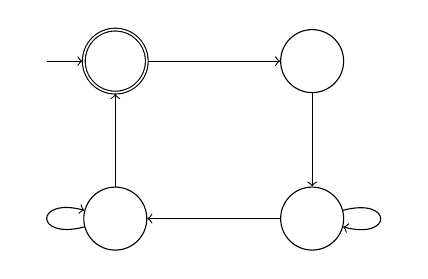
\begin{tikzpicture}[initial text={}]
\newcommand{\x}{2.5}
\node[state,accepting,initial] (q1) at (0,0) {};
\node[state] (q2) at (\x,0) {};
\node[state] (q5) at (\x,-2) {};
\node[state] (q6) at (0,-2) {};

\draw[->] (q1) to node[above]  {} (q2);
\draw[->] (q2) to node[right]  {} (q5);
\draw[->, loop right] (q5) to node[right]  {} (q5);
\draw[->] (q5) to node[above]  {} (q6);
\draw[->, loop left] (q6) to node[left]  {} (q6);
\draw[->] (q6) to node[left]  {} (q1);
\end{tikzpicture}
\end{center}
\caption{The automaton  computing the maximal difference between the lengths of blocks of 's at odd and the following even positions.}\label{fig:autDiff}
\end{figure}

The automaton  has a single initial state , which is also the only accepting state.
It processes the word  in subwords  in the following way.
First, it reads  upon which it takes transitions from  to  and from  to , where it  starts counters  and .
Next, it moves to the state  where it counts letters  incrementing counter  and decrementing counter .
Then, upon reading , it moves to , where it counts letters , but it decrements counter  and increments counter .
After reading  the value of counter  is  and counter  is .
In the following transition from  to , the automaton terminates both counters.
The aggregating function  of  is , thus the automaton discards the lower value, i.e.,
the value of  is  and the automaton computes the supremum over values of all blocks.
It follows that the value of  is .
\end{exa}


\subsection{Nested weighted automata}
In this section we describe nested weighted automata introduced in~\cite{nested},
and closely follow the description of~\cite{nested}.
For more details and illustrations of such automata we refer the reader
to~\cite{nested}.
We start with an informal description.


\smallskip
\noindent{\em Informal description.}
A \emph{nested weighted automaton} consists of a labeled automaton over infinite words,
called the \emph{master automaton}, a value function  for infinite words,
and a set of weighted automata over finite words, called \emph{slave automata}.
A nested weighted automaton can be viewed as follows:
given a word, we consider the run of the master automaton on the word,
but the weight of each transition is determined by dynamically running
slave automata; and then the value of a run is obtained using the
value function .
That is, the master automaton proceeds on an input word as an usual automaton,
except that before it takes a transition, it starts a slave automaton
corresponding to the label of the current transition.
The slave automaton starts at the current position in the word of the master automaton
and works on some finite part of the input word. Once the slave automaton finishes,
it returns its value to the master automaton, which treats the returned
value as the weight of the current transition that is being executed.
The slave automaton might immediately accept and return value ,
which corresponds to \emph{silent} transitions.
If one of slave automata rejects, the nested weighted automaton rejects.
We define this formally as follows.

\smallskip

\Paragraph{Nested weighted automata}.
A \emph{nested weighted automaton} (NWA)  is a tuple

such that

\begin{enumerate}
\item , called the \emph{master automaton}, is a -labeled automaton over infinite words
(the labels are the indexes of automata ),
\item  is a value function on infinite words, called the \emph{master value function}, and
\item  are weighted automata over finite words called \emph{slave automata}.
\end{enumerate}
\smallskip

\noindent Intuitively, an NWA can be regarded as an -automaton whose weights are dynamically computed at every step by the corresponding slave automaton.
We define an \emph{-automaton} as an NWA where the master value function is  and all slave automata are -automata.

\smallskip
\Paragraph{Semantics: runs and values}.
A \emph{run} of an NWA  on an infinite word  is an infinite sequence
 such that
(1)~ is a run of  on ;
(2)~for every  we have  is a run of the automaton ,
referenced by the label  of the master automaton, on some finite subword  of the input word .
The run  is \emph{accepting} if all
runs  are accepting (i.e.,  satisfies its acceptance
condition and each  ends in an accepting state)
and infinitely many runs of slave automata have length greater than  (the master automaton takes infinitely many non-silent transitions).
The value of the run  is defined as
, where  is the value of the run  in
the corresponding slave automaton.
The value of a word  assigned by the automaton , denoted by
, is the infimum of the set of values of all \emph{accepting} runs.
We require accepting runs to contain infinitely many non-silent transitions because
 is a value function over infinite sequences, so we need
the sequence  with  symbols removed to be infinite.

\smallskip
\Paragraph{Deterministic nested weighted automata}. An NWA  is \emph{deterministic} if (1)~the master automaton
and all slave automata are deterministic, and (2)~in all slave automata
accepting states have no outgoing transitions.
Condition (2) implies that no accepting run of a slave automaton visits an accepting state twice.
Intuitively, slave automata have to accept the first time they encounter an accepting state as
they will not reach an accepting state again.

\smallskip
\Paragraph{Bounded width.} An NWA has \emph{width}  if and only if  is the minimal number such that
in every accepting run at every
position at most  slave automata are active.


\begin{exa}[Average response time with bounded requests]\label{ex:NWA}
Consider an alphabet  consisting of requests , grants  and idle instructions .
The average response time (ART) property asks for the average number of instructions between
any request and the following grant. It has been shown in~\cite{nested} that NWA can express ART\@.
However, the automaton from~\cite{nested} does not have bounded width.
To express the ART property with NWA of bounded width we consider only words such that between any two grants there are at most  requests.

Average response time over words where between any two grants there are at most  requests can be expressed by a -automaton
. Such an automaton  is depicted in Fig.~\ref{fig:ART-k}.
The master automaton of  accepts only words with  infinite number of requests and grants, where every grant is followed by a request and
there are at most  requests between any two grants.
On letters  and , the master automaton invokes a dummy automaton , which immediately accepts;
the result of invoking such an automaton is equivalent to taking a silent transition as
the automaton  returns , the empty value.
On letters , denoting requests, the master automaton invokes , which
counts the number of letters to the first occurrence of letter , i.e.,
the automaton  computes the response time for the request on the position it is invoked.
The automaton  computes the limit average of all returned values, which is precisely
ART (on the accepted words).
Note that the width of  is .


\begin{figure}
\centering
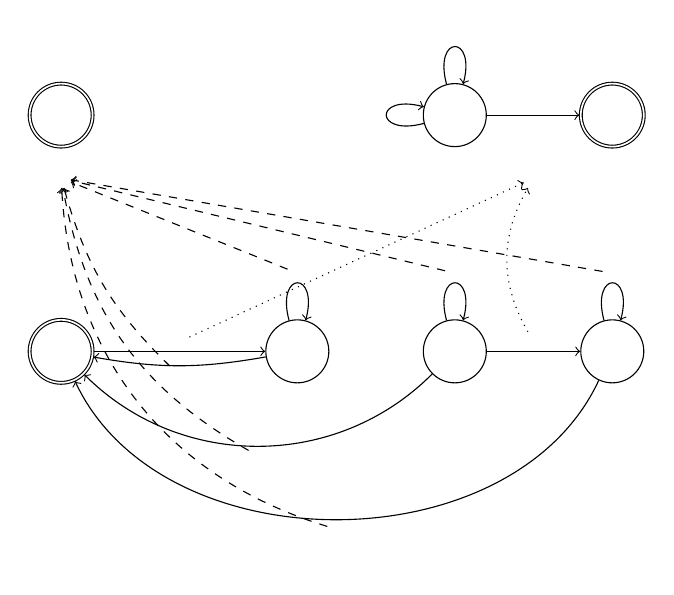
\begin{tikzpicture}
\newcommand{\x}{2.0}
\node[state,accepting] (q0) at (-1,0) {};
\node[state] (q1) at (\x,0) {};
\node[state, inner sep =1pt] (q2) at (2*\x,0) {};
\node[state] (q3) at (3*\x,0) {};

\node at (1.5*\x,0) {};

\draw[->, loop above] (q1) to node[above] (e2) {} (q1);
\draw[->, loop above] (q2) to node[above] (e3) {} (q2);
\draw[->, loop above] (q3) to node[above] (e4) {} (q3);

\draw[->,bend left=10] (q1) to node[below] (e5) {} (q0);
\draw[->,bend left=45] (q2) to node[below] (e6) {} (q0);
\draw[->,bend left=65] (q3) to node[below] (e7) {} (q0);


\draw[->] (q0) to node[above] (e8) {} (q1);
\draw[->] (q2) to node[above] (e9) {} (q3);


\node at (5.5,-1.5) {};

\begin{scope}[yshift=3cm]
\node[state,accepting] (q00) at (-1,0) {};

\node (A1) at (-1,-0.8) {};

\node[state] (q10) at (4,0) {};
\node[state,accepting] (q11) at (6,0) {};

\node (A2) at (5,-0.8) {};

\draw[->] (q10) to node[above] {} (q11);
\draw[->, loop above] (q10) to node[above] {} (q10);
\draw[->, loop left] (q10) to node[left] {} (q10);
\end{scope}

\draw[->, dashed] (e2) to (A1);
\draw[->, dashed] (e3) to (A1);
\draw[->, dashed] (e4) to (A1);
\draw[->, dashed, bend left = 15] (e5) to (A1);
\draw[->, dashed, bend left = 25] (e6) to (A1);
\draw[->, dashed, bend left = 35] (e7) to (A1);

\draw[->, dotted] (e8) to (A2);
\draw[->, dotted, bend left = 30] (e9) to (A2);

\end{tikzpicture}
\caption{The -automaton computing the average response time over words with infinite number of requests and grants such that between any two
grants there are at most  requests.}\label{fig:ART-k}
\end{figure}
\end{exa}


\subsection{Translation}
We now present translations from NWA to automata with monitor counters and vice-versa. To state correctness of translation, we first define equivalence.

\Paragraph{Equivalence of quantitative automata}. We say that , each being a weighted automaton, an automaton with monitor counters or an NWA over infinite words from , are \emph{equivalent}
 if and only if for all words  we have
.

Now, we state the main translation lemma:


\begin{restatable}[Translation Lemma]{lem}{MCvsNested}\label{l:mc-vs-nested}
For every value function  on infinite words we have the following:
\begin{enumerate}
\item Every deterministic -automaton with monitor counters  can be transformed in polynomial time
into an equivalent deterministic -automaton of bounded width.
\item Every non-deterministic (resp., deterministic) -automaton of bounded width can be transformed in exponential time
into an equivalent non-deterministic (resp., deterministic) -automaton with monitor counters.
\end{enumerate}
\end{restatable}

\noindent
Before the formal proof, we illustrate below the key ideas of the above translations of
Lemma~\ref{l:mc-vs-nested} to automata from Examples~\ref{ex:AMC}~and~\ref{ex:NWA}.

\begin{exa}[Translation of automata with monitor counters to nested weighted automata]
Consider a deterministic automaton  with  monitor counters.
We construct an NWA  equivalent to .
The automaton  uses  slave automata to track values of  monitor counters in the following way.
The master automaton of  simulates ; it invokes slave automata whenever  starts monitor counters.
Slave automata simulate  as well. Each slave automaton is associated with some counter ; it starts in the state (of ) the counter  is initialized,
simulates the value of counter , and terminates when counter  is terminated.
Figure~\ref{fig:AMCtoNWA} presents the result of transition of  the automaton  from Example~\ref{ex:AMC}
to a -automaton of width bounded by .

\begin{figure}
\centering
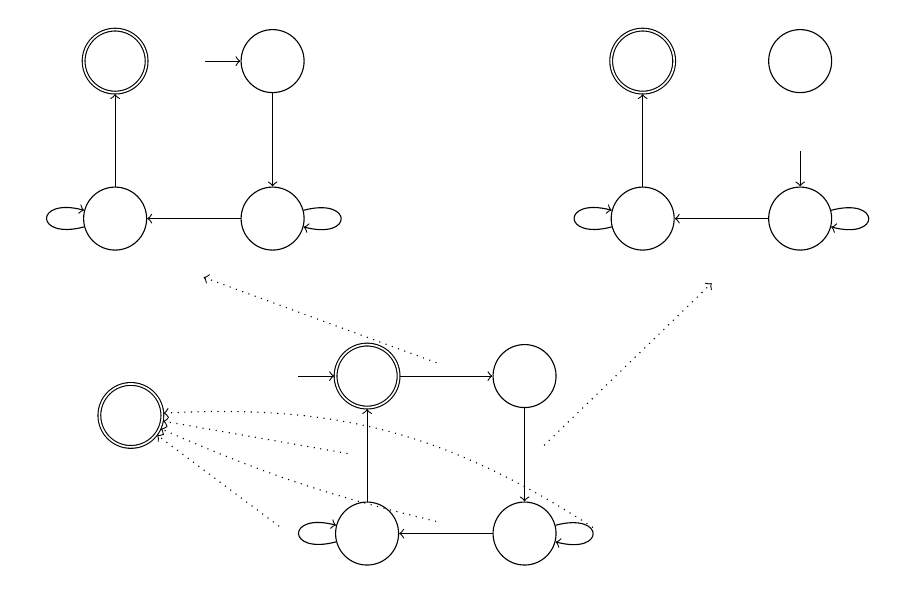
\begin{tikzpicture}[initial text={}]
\newcommand{\x}{1.0}

\begin{scope}[yshift=4cm,xshift=-3.2cm]
\node[state,accepting] (q11) at (0,0) {};
\node[state,initial] (q12) at (2*\x,0) {};
\node[state] (q15) at (2*\x,-2) {};
\node[state] (q16) at (0,-2) {};

\draw[->] (q12) to node[right]  {} (q15);
\draw[->, loop right] (q15) to node[right]  {} (q15);
\draw[->] (q15) to node[above]  {} (q16);
\draw[->, loop left] (q16) to node[left]  {} (q16);
\draw[->] (q16) to node[left]  {} (q11);

\node (A1) at (1,-2.7) {};

\end{scope}


\begin{scope}[yshift=4cm,xshift=3.5cm]
\node[state]  at (2*\x,0) {};
\node[state,accepting] (q21) at (0,0) {};
\node[state,initial above] (q25) at (2*\x,-2) {};
\node[state] (q26) at (0,-2) {};

\draw[->, loop right] (q25) to node[right]  {} (q25);
\draw[->] (q25) to node[above]  {} (q26);
\draw[->, loop left] (q26) to node[left]  {} (q26);
\draw[->] (q26) to node[left]  {} (q21);
\node (A2) at (1,-2.7) {};
\end{scope}


\node[state,accepting] (A3state)  at (-3,-0.5) {};
\node (A3) at (-3,-1.3) {};



\node[state,accepting,initial] (q1) at (0,0) {};
\node[state] (q2) at (2*\x,0) {};
\node[state] (q5) at (2*\x,-2) {};
\node[state] (q6) at (0,-2) {};

\draw[->] (q1) to node[above] (e1) {} (q2);
\draw[->] (q2) to node[right] (e2) {} (q5);
\draw[->, loop right] (q5) to node[right] (e3) {} (q5);
\draw[->] (q5) to node[above] (e4) {} (q6);
\draw[->, loop left] (q6) to node[left] (e5)  {} (q6);
\draw[->] (q6) to node[left] (e6) {} (q1);

\draw[->,dotted] (e1) to (A1);
\draw[->,dotted] (e2) to (A2);

\draw[->,dotted, bend right=18] (e3) to (A3state);
\draw[->,dotted, bend left=5] (e4) to (A3state);
\draw[->,dotted] (e5) to (A3state);
\draw[->,dotted] (e6) to (A3state);


\end{tikzpicture}
\caption{A nested weighted automaton resulting from translation of the automaton  from Example~\ref{ex:AMC}.
The master automaton is obtained from  (see Figure~\ref{fig:autDiff}) by changing the labels of transitions.
All slave automata are defined based on ; each slave automaton corresponds to  starting in a state , in which a counter  is initialized, and contains all the transitions that can be taken before
the counter  is terminated.}\label{fig:AMCtoNWA}
\end{figure}
\end{exa}

\begin{exa}[Translation of nested weighted automata of bounded width to automata with monitor counters]
Consider an -automaton  of width bounded by .
We construct an automaton with monitor counters , which
simulates the master automaton and up to  slave automata running in parallel.
To simulate values of slave automata it uses monitor counters, each counter separately for each slave automaton.

Figure~\ref{fig:NWAtoAMC} shows the result of translation of  the automaton  from Example~\ref{ex:NWA}
to the automaton with monitor counters . The set of states of  there is
, i.e.,
the states of the master automaton and all non-accepting states of slave automata (in deterministic NWA accepting states are sink states, hence storing them is redundant).
Now, observe that only reachable states of  are , i.e., the reachable part of
 is isomorphic (in the sense of graphs) to the master automaton of .

\begin{figure}
\centering
\begin{tikzpicture}
\newcommand{\x}{2.8}
\node[state] (q0) at (-1,0) {};
\node[state] (q1) at (\x,0) {};
\node[state, inner sep =1pt] (q2) at (2*\x,0) {};
\node[state] (q3) at (3*\x,0) {};

\node at (1.5*\x,0) {};


\draw[->, loop above] (q1) to node[above] (e2) {} (q1);
\draw[->, loop above] (q2) to node[above] (e3) {} (q2);
\draw[->, loop above] (q3) to node[above] (e4) {} (q3);


\draw[->,bend left=10] (q1) to node[below] (e5) {} (q0);
\draw[->,bend left=45] (q2) to node[below] (e6) {} (q0);
\draw[->,bend left=65] (q3) to node[below] (e7) {} (q0);


\draw[->,bend left=10] (q0) to node[above] (e8) {} (q1);
\draw[->] (q2) to node[above] (e9) {} (q3);
\node at (0.5,1.5) {};
\end{tikzpicture}
\caption{The (reduced) result of translation of the automaton  from  Example~\ref{ex:NWA} to an automaton with monitor counters. All vectors have dimension .
Vector  denotes the vector with all components equal .
Vector  denotes the whose -th component is  and other components are .
Vector  denotes the vector whose components  are  and the remaining components are .
}\label{fig:NWAtoAMC}
\end{figure}
\end{exa}

\begin{proof}[Proof of Lemma~\ref{l:mc-vs-nested}]
\Paragraph{(Translation of automata with monitor counters to NWA)}:
Consider a deterministic -automaton  with  monitor counters and the set of states .
We define an -automaton , which consists of a master automaton  and
slave automata .
The slave automaton  is a dummy automaton, i.e., it has only a single state which is both
the initial and the accepting state. Invoking such an automaton is equivalent to taking a silent transition (with no weight).
Next, the master automaton  and slave automata 
are variants of , i.e., they share the underlying transition structure.
The automaton  simulates , i.e., it has the same states and the transitions among these states as .
However, whenever  activates counter , the master automaton invokes the slave automaton , where  is their current state (both  and the simulated ).
The accepting condition of  is the same as of .
We can construct  in polynomial time in .
For every , the slave automaton 
keeps track of counter , i.e., it
simulates  and applies instructions of  for counter 
to its value. That is, whenever  changes the value of counter  by , the automaton 
takes a transition of the weight . Finally,  terminates precisely when  terminates counter .
The automaton  can be constructed in polynomial time in .
There are at most  such slave automata and each of them has the size bounded by .
Therefore,  is polynomial in  and can be constructed in polynomial time in .

The semantics of automata with monitor counters implies that  accepts if and only if  accepts and, for every word,
the sequences of weights produced by the runs of  and  on that word coincide. Therefore,
the values of  and  coincide on every word.


\Paragraph{(Translation of NWA of bounded width to automata with monitor counters)}: We show that non-deterministic (resp., deterministic)
-automata with monitor counters  subsume
non-deterministic (resp., deterministic) -automata of bounded width.
Consider a non-deterministic -automaton  with width bounded by .
We define an -automaton  with  monitor counters that works as follows.
Let  be the set of states of the master automaton of  and  be the union of the sets of states of the slave automata of .
The set of states of  is .
The automaton  simulates runs of the master automaton and slave automata by keeping track of the state of the master automaton and
states of up to  active slave automata. If there are less than  active slave automata,  uses  to mark slots that can be used in the future to simulate slave automata.
Moreover, it uses counters to simulate the values of slave automata, i.e.,
whenever a slave automaton is activated,  simulates the execution of this automaton and
assigns some counter  to that automaton.
Next, when the simulated slave automaton takes a transition of the weight  the automaton 
changes the value of counter  by .
Finally,  terminates counter  when the corresponding slave automaton terminates.
The size of  is bounded by  and it can be constructed in time .

Since  has width bounded by , the simulating automaton  never runs out of counters to simulate slave automata.
Moreover, as it simulates runs of the master automaton and slave automata of , there is a one-to-one
correspondence between runs of  and runs of  and accepting runs of  correspond to accepting runs of .
Finally, the sequence of weights for the master automaton determined by a given run of  coincides with the sequence of
weights of  on the corresponding run. Therefore, the values of  and  coincide on every word.
Thus, non-deterministic -automata with monitor counters  subsume
non-deterministic -automata of bounded width.

Now, assume that  is deterministic. Therefore, the master automaton and all slave automata are deterministic and accepting states of slave automata have no outgoing transitions.
We claim that  is deterministic as well.
Consider a state  from  and every letter .
The successor over  of  is uniquely determined as the master automaton is deterministic.
For all , which are not accepting, the successor states of deterministic slave automata are uniquely determined.
If some state  is accepting, then the slave automaton has no outgoing transition and the successor state is .
Finally, for  equal , the one with the least index becomes the initial state of the newly invoked slave automaton and
the other states remain .
Therefore, the automaton  is deterministic.
\end{proof}

A direct consequence of Lemma~\ref{l:mc-vs-nested}  is the following theorem:

\begin{thm}\label{th:equivalence}
For every  , deterministic
bounded-width -automata and deterministic -automata with monitor counters are expressively equivalent.
\end{thm}

\begin{rem}[Discussion]
Theorem~\ref{th:equivalence}
 states that deterministic automata with monitor counters have
the same expressive power as deterministic NWA of bounded width. However, the latter may be exponentially more succinct.
In consequence, lower bounds on deterministic automata with monitor counters imply lower bounds on NWA of bounded width.
Conversely, deterministic NWA can be considered as automata with infinite number of monitor counters, therefore
upper bounds on deterministic NWA imply upper bounds on deterministic automata with monitor counters
\end{rem}


\section{Problems}
\subsection{Classical questions}

The classical questions in automata theory are \emph{emptiness} and \emph{universality} (of a language).
These problems have their counterparts in the quantitative setting of weighted automata and their extensions.
The (quantitative) emptiness and universality problems are defined in the same way for weighted automata, NWA and automata with monitor counters, i.e.,
in the following definition the automaton  can be a weighted automaton, an NWA or an automaton with monitor counters.
\begin{itemize}
\item \textbf{Emptiness}: Given an automaton  and , decide whether there is a word  with
?
\item \textbf{Universality}: Given an automaton  and  , decide whether for all words  we have
?
\end{itemize}
The universality question asks for \emph{non-existence} of a word  such that .

\subsection{Probabilistic questions}
The classical questions ask for the (non-)existence of words for input automata, whereas in the probabilistic setting, input automata are analyzed w.r.t.
a probability distribution.
We consider probability distributions over infinite words , and as a finite representation
consider the classical model of Markov chains.

\smallskip
\Paragraph{Labeled Markov chains}.
A \emph{(labeled) Markov chain} is a tuple ,
where  is the alphabet of letters,
 is a finite set of states,  is an initial state,
 is the edge probability function, which
for every  satisfies that .

\smallskip
\Paragraph{Distributions given by Markov chains}.
Consider a Markov chain . For every finite word , the probability of , denoted ,
w.r.t.\ the Markov chain  is the sum of probabilities of paths labeled by ,
where the probability of a path is the product of probabilities of its edges.
For basic open sets ,
we have , and then the
probability measure over infinite words defined by  is the unique
extension of the above measure (by Carath\'{e}odory's extension theorem~\cite{feller}).
We will denote the unique probability measure defined by  as , and
the associated expectation measure as .

We define \emph{the uniform probability measure}  such that for every  we have
. It can be defined by a single-state Markov chain, in which
all transitions are self-loops labled with the same probability .

\smallskip
\Paragraph{Automata as random variables}.
Note that deterministic weighted automata,  NWA or automata with monitor counters
all define functions , which are measurable with respect to probability measures given by Markov chains, and hence
these functions can be interpreted as random variables.
Therefore, given an automaton  and a Markov chain , we consider the following fundamental quantities:
\begin{enumerate}
\item \textbf{Expected value}:  is the expected value of
the random variable defined by the automaton  w.r.t.\ the probability measure defined by the Markov chain .
\item \textbf{(Cumulative) distribution}:  is the
cumulative distribution function of
the random variable defined by the automaton  w.r.t.\ the probability measure defined by the Markov chain .
\end{enumerate}

\smallskip
\Paragraph{Computational questions.}
Given an automaton  and a Markov chain , we consider the following basic
computational questions:
\begin{enumerate}[label={(Q\arabic*)}]
\item The \emph{expected question} asks to compute  .
\item The \emph{distribution question} asks, given a threshold , to compute .
\end{enumerate}
\smallskip
Questions (Q1) and (Q2) have their approximate variants, which, given an additional input , ask to compute values that are -close to
 or , i.e., given :
\begin{enumerate}[resume,label={(Q\arabic*)}]
\item The \emph{approximate expected question} asks to compute a value  such that , and
\item The \emph{approximate distribution question} asks to compute a value  such that .
\end{enumerate}
\smallskip
Additionally, a special important case for the distribution question is
\begin{enumerate}[resume,label={(Q\arabic*)}]
\item The \emph{almost-sure distribution question} asks whether for a given  the probability  is exactly .
\end{enumerate}

\noindent
We refer to questions (Q1)--(Q5) as \emph{probabilistic questions}. Note that an upper bound on the complexity of the expected and distribution questions imply the same upper bound on all probabilistic questions as approximate and almost-sure variants are special cases.

\begin{exa}[Expected average response time]
Consider an NWA  from Example~\ref{ex:NWA}. Recall that it computes ART on words it accepts (bounded number of requests between any two grants).
Next, consider a Markov chain  which gives a distribution on words over .
In such a case, the value  is the expected ART\@.
\end{exa}



\section{Results on classical questions}
	\smallskip\noindent{\bf Existing results.}
The complexity of the classical decision problems for NWA
has been established in~\cite{nested} which is presented in Table~\ref{tab1}.
\begin{table}[t]
\centering
\def\tabcolsep{5pt}
\begin{tabular}{|c|c|c|c|c|} \hline \multicolumn{2}{|c|}{}& &  & \multirow{2}{*}{} \\
\multicolumn{2}{|c|}{}&  &   & \\
\hline  &Empt.&
\multicolumn{3}{|c|}{ {-comp.}}  \\
\cline{2-2}
\cline{4-4}
 &Univ.&  &\PTIME&  \\
\hline \multirow{2}{*}{} & Empt. &
\multicolumn{2}{|c|}{ {-comp.}} &
\multirow{2}{*}{ } \\
\cline{2-2}
\cline{4-4}
&Univ. & &\PTIME&    \\
\hline \multirow{2}{*}{} & Empt. & \multirow{2}{*}{-comp.}  & Undecidable & Open \\
\cline{2-2}
\cline{4-4}
& Univ. &  &   &  \\
\hline \end{tabular}
\caption{Decidability and complexity of emptiness and universality for deterministic -automata.
Functions  are listed in the first row and functions  are in the first column.
}\label{tab1}
\end{table}

\smallskip\noindent{\bf New results}.
Due to Lemma~\ref{l:mc-vs-nested},
decidability of deterministic -automata implies decidability of
deterministic automata with monitor counters with the value function .
However, the undecidability result of NWA does not imply undecidability for
automata with monitor counters as the NWA in the reduction may have unbounded width.
We present the undecidability result for NWA of bounded width, which implies undecidability of the emptiness problem for automata with monitor counters.
Thus, our following result completes the decidability picture also for automata with monitor counters
(i.e., the decidability results coincide with the  row of Table~\ref{tab1}).

\begin{thm}\label{th:undecidable-limsup}
The emptiness problem is undecidable for deterministic -automata (resp., -automata) with  monitor counters.
\end{thm}
\begin{proof}
We show undecidability of the emptiness problem for  deterministic -automata of width .
The proof for deterministic -automata is virtually the same.
Then, the theorem follows from the translation lemma (Lemma~\ref{l:mc-vs-nested}).


We show a reduction from the halting problem for deterministic two-counter machines, which is undecidable~\cite{minsky1961recursive}.
Let  be a deterministic two-counter machine and let  be the set of states of .
We define a deterministic -automaton  of width  such that
 has a run of the value not exceeding  if and only if  has an accepting computation.

Consider the alphabet \}\M\#\Mqxyq 1^{x} 2^{y}\M\,   checks consistency of the transitions by checking two conditions: (C1)~Boolean consistency, and (C2)~counter consistency.
The condition (C1) states that encoded subsequence configurations, which are represented by subwords  ,
 are consistent with the transition function of  modulo counter values, i.e., under counter abstraction to values  and ``strictly positive''.
Observe that a finite automaton can check that. The conditions that need to be checked are as follows:
(C1-1)~Boolean parts of transitions are consistent; the automaton checks only emptiness/nonemptiness of counters and based on that verifies whether a subword  is valid w.r.t.\ transitions of .
For example, consider transition  of  stating that ``if  is in state , the first counter
is  and the second counter is positive, then change the state to  increment the first counter and
decrement the second one''. This transition corresponds to the regular expression
.
(C1-2)~The initial and final configurations in each computation (between q_I 1^0 2^0q_f 1^0 2^0\
\lim_{n \to \infty} \frac{|\Path[1,n]|_{e_i} }{|\Path[1,n]|_{e_1} + \cdots + |\Path[1,n]|_{e_k}} = x[e_i].
\label{eq:correctness-silent}

x[(s,a,s')] = E(s,a',s') \cdot \sum_{s'' \in S_{\silentMarkov}, a' \in \Sigma} x[(s'',a',s)],
 \sum_{i=1}^{N-1} {\left(\frac{1}{2}\right)}^{i} \cdot i + N \sum_{i=N}^{\infty} {\left(\frac{1}{2}\right)}^i = 	2 - (N-1)\cdot {\left(\frac{1}{2}\right)}^{N-1} + N \cdot  {\left(\frac{1}{2}\right)}^{N-1} = 2 -  {\left(\frac{1}{2}\right)}^{N-1}.
    \min(N,k), \min(N,k-1), \ldots, 2, 1,

    1,2, \ldots, \min(N,k-1), \min(N,k).

\expected_{\markov}(\nestedA) = \expected_{\markov}(\nonnestedA) = \expected (\markov_E) = \expected(\markov_R) = \expected(\MCfromNested)

x[e_1] + \cdots + x[e_k] = x[e_1']+ \cdots +x[e_l'].
 c(e_1) \cdot x[e_1] + \cdots + c(e_k) \cdot x[e_k] =
 c'(e_1') \cdot x[e_1'] + \cdots + c'(e_l') \cdot x[e_l'],

 c'(e_1') \cdot x[e_1'] + \cdots + c'(e_l') \cdot x[e_l'] = \sum_{i=1}^k c(e_i) \cdot \big(x[e_1'] \cdot p(e_1',e_i) + \cdots + x[e_l'] \cdot  p(e_l',e_i)\big)

x[e_1'] \cdot  p(e_1',e_i) + \cdots + x[e_l']\cdot   p(e_l',e_i) = x[e_i].
 c(e_1) \cdot x[e_1] + \cdots + c(e_k) \cdot x[e_k] =
 c'(e_1') \cdot x[e_1'] + \cdots + c'(e_l') \cdot x[e_l']

\lim_{N \rightarrow \infty} \probability_{\markov}(\{ w \mid |\valueL{\nestedA}(w) - \valueL{\nestedA^N}(w)| \geq \epsilon \}) = 0

\valueL{\nestedA^N}(w) - C \cdot \valueL{\excessA{N}}(w) \leq \valueL{\nestedA}(w) \leq \valueL{\nestedA^N}(w) + C \cdot \valueL{\excessA{N}}(w).

\probability_{\markov}(\{ w \mid |\valueL{\nestedA}(w) - \valueL{\nestedA^N}(w)| \geq \epsilon \}) =
\probability_{\markov}(\{ w \mid |\valueL{\excessA{N}}(w)| \geq \frac{\epsilon}{C} \})

\text{(*)}\quad \expected_{\markov}(\excessA{N}) \leq \sum_{K \geq N} \sum_{i=0}^{K-1} \expected_{\markov}(\partialExcessA{K,i}).

is  if and only if  encodes a valid and accepting computation of .
Otherwise, the supremum is at least .
Thus, in our case, the infimum over the values of slave automata is  if and only if 
encodes a valid and accepting computation of . Otherwise,
the value of  is at most .
Therefore,   if and only if  does not have an accepting computation.

\Paragraph{(2)}: We show that knowing how to compute the expected value of deterministic
-automata, we can decide equality in the distribution question.
Let  be an automaton and we ask whether .
We construct another automaton  that simulates , but at the first transition it invokes a slave automaton that returns the value .
The values of automata  and  differ precisely on words which have values (assigned by ) greater than .
Thus, their expected values
 and  differ if and only if
 is different than . Due to undecidability of the latter problem, there exists no Turing machine that computes the expected value of -automata
over the uniform distribution.
\end{proof}



Finally, we have the following result for the absolute sum value function, which guarantees that the return values are at least . We present a slightly more general result.
Recall that we assume that weights in slave automata are given in unary.

\begin{lem}\label{l:bound-from-below}
Given a Markov chain , a value  and a deterministic -automaton
such that the value of every slave automaton is bounded from below,
the values  and  can be computed in exponential time in  and polynomial time in .
\end{lem}



\begin{proof}
Consider a deterministic -automaton  such that the value of every slave automaton is bounded from below.
Let  and let  be  considered as a deterministic -automaton.
We show that on almost all words  we have .
Then,

and  and the values
 and  can be computed in exponential time by
Lemma~\ref{l:infSolutions} taking into account the remark about  being input.

Since the value of every slave automaton  is bounded from below,
the (reachable part of) the weighted Markov chain  considered as a weighted graph does not have negative cycles.
Therefore, the minimal value  can achieve is greater than .
Moreover, every accepting run of  ends up in some SCC of , where
almost all words have the same value~(Lemma~\ref{l:in-scc-all-equal}), which
is either  (if almost all words are rejected) or bounded from above by . This value can be computed in polynomial time.
Therefore, the value of almost all words belong to the interval  or it is  if the run on  on this word is rejecting.
Finally, the sets of words with accepting runs in  and  coincide.
\end{proof}

The above lemma implies that the probabilistic questions for deterministic -automata can be answered in exponential time in  and polynomial time in .
Note that -automata and -automata are not dual.
Indeed, in Lemma~\ref{l:sup-to-inf} we multiply weights by , which turns -automata into -automata with negative weights.
Thus, we consider separately the distribution question for -automata.
We show that the distribution question for deterministic -automata is
decidable in .



\begin{lem}\label{l:distributionSumPlusDecidable}
The distribution question for deterministic -automata can be computed in exponential time in  and polynomial time in .
\end{lem}
\begin{proof}
Let  be a deterministic -automaton,  be a Markov chain and let  be a threshold in the distribution question.
Consider  defined as  considered as a -automaton with .
Observe that for every word  we have  if and only if
. Therefore,
.
The latter value can be computed in exponential time in  and polynomial time in  (Lemma~\ref{l:infSolutions}).
\end{proof}



\begin{thm}\label{th:compInf}
Let .
The complexity results for the probabilistic questions for -automata
and -automata are summarized in Table~\ref{tab:compInf}, with the exception
of the expected question of -automata.
\end{thm}

\begin{table}[ht]
\centering
\begin{tabular}{|c|c|c|c|} \hline & , , & \multirow{2}{*}{} \\
&  &  \\
\hline Expected value & \multirow{3}{*}{~(Lemma~\ref{l:infSolutions},~\ref{l:infSumSolution},~\ref{l:distributionSumPlusDecidable})} & \multirow{3}{*}{\uncomp}\\
\cline{1-1}
{Distribution} & \multirow{3}{*}{-hard~(Lemma~\ref{l:hardness-for-det-inf})} & \multirow{3}{*}{(Lemma~\ref{l:inf-prob-undec})}\\
\cline{1-1}
Almost sure & &  \\
distribution &  & \\
\hline Approximate: & \multicolumn{2}{|c|}{\multirow{2}{*}{~(Lemma~\ref{l:infSolutions},~\ref{l:infSumSolution})}} \\
(a)~expected value & \multicolumn{2}{|c|}{\multirow{2}{*}{\#P-hard~(Lemma~\ref{l:hardness-for-det-inf})}} \\
(b)~distribution & \multicolumn{2}{|c|}{} \\
\hline \end{tabular}
\caption{The complexity results for various problems for deterministic NWA with  and  value functions,
with exception of the expected question of -automata which is open.
Columns represent slave-automata value functions, rows represent probabilistic questions.
}\label{tab:compInf}
\end{table}



\smallskip\noindent{\em Open question}.
The decidability of the expected question of -automata is open.
This open problem is related to the language inclusion problem of deterministic
-automata which is also an open problem.

\begin{rem}[Contrast with classical questions]\label{remark:Inf-classical-vs-probabilistic}
Consider Table~\ref{tab1} for the classical questions and
our results established in Table~\ref{tab:compInf} for probabilistic questions.
There are some contrasting results, such as, while for
-automata the emptiness problem is undecidable,
the approximation problems are decidable.
\end{rem}


\begin{rem}[Contrast of  vs ]\label{remark:LimInf-vs-Inf}
We remark on the contrast of the  vs  value functions.
For the classical questions of emptiness and universality, the complexity and
decidability always coincide for  and  value functions for NWA
(see Table~\ref{tab1}).
Surprisingly we establish that for probabilistic questions there is a substantial
complexity gap: while the  problems can be solved in polynomial time, the
 problems are undecidable, -hard, and even -hard for approximation.
\end{rem}

\section{Results on non-deterministic automata}\label{s:nondeterminism}
In this section, we briefly discuss non-deterministic NWA evaluated on Markov chains.
First, we discuss the definition of random variables defined by non-deterministic NWA\@. Next, we present two negative results.

\smallskip\noindent{\em Non-deterministic NWA as random variables}.
A non-deterministic NWA  defines a function  as in the deterministic case via
.
Recall that , where  is the set of accepting runs of  on .
We show that  is measurable w.r.t.\ any probability measure given by a Markov chain.
It suffices to show that for every interval , its preimage  is measurable.
Consider a set  of words with runs of  of
the value at most . More precisely, let  be the the master value function of .
     Then,  if and only if
(1)~ is a run of the master automaton of  on ,
(2)~for every , the slave automaton invoked by the master automaton at position  has a finite run on  of the value
,
(3)~.
Observe that  is a Borel set in the product topology. The preimage  is
the projection of the Borel set , and hence it is an \emph{analytic set}, which is measurable~\cite{kechris}.




\smallskip\noindent{\em Conceptual difficulty}.
The evaluation of a non-deterministic (even non-nested) weighted automaton over a Markov
chain is conceptually different as compared to the standard model of
Markov decision processes (MDPs).
Indeed, in an MDP, probabilistic transitions are interleaved with non-deterministic transitions,
whereas in the case of an automaton, it runs over a word that has been already generated by
the Markov chain.
In MDPs, the strategy to resolve non-determinism can only rely on the past, whereas
in the automaton model the whole future is available (i.e., there is a crucial distinction
between online vs offline processing of the word).
Below we present an example to illustrate
this conceptual problem.

\begin{exa}
Consider a non-deterministic -automaton , depicted in Figure~\ref{fig:nondet-vs-MDP}.
Intuitively, the automaton processes a given word in blocks of letters  separated by letters .
At the beginning of every block it decides whether the value of this block is
the number of  letters  minus the number of  letters  divided by 
(i.e., ) or
the opposite (i.e., ).
\begin{figure}
\centering
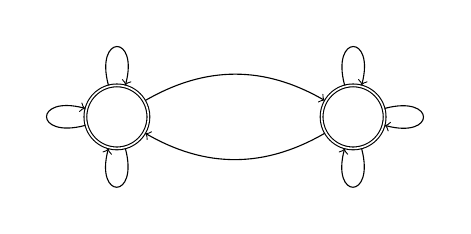
\begin{tikzpicture}

\node[state,accepting] (Q0) at (0,0) {};
\node[state,accepting] (Q1) at (3,0) {};

\draw[->,loop left] (Q0) to node[left]{} (Q0);
\draw[->,loop above] (Q0) to node[above]{} (Q0);
\draw[->,loop below] (Q0) to node[below]{} (Q0);

\draw[->,loop right] (Q1) to node[right]{} (Q1);
\draw[->,loop above] (Q1) to node[above]{} (Q1);
\draw[->,loop below] (Q1) to node[below]{} (Q1);

\draw[->,bend left] (Q0) to node[above]{} (Q1);
\draw[->,bend left] (Q1) to node[below]{} (Q0);
\end{tikzpicture}
\caption{An example of non-deterministic automaton, in which non-deterministic choices has to ``depend on the future'' in order to obtain the infimum.}\label{fig:nondet-vs-MDP}
\vspace{-1em}
\end{figure}
Let  be the uniform distribution on infinite words over .
Suppose that the expected value of  w.r.t.  is evaluated as in MDPs case, i.e.,
non-deterministic choices depend only on the read part of the word.
Then, since the distribution is uniform, any strategy results in the same expected value, which is equal to .
Now, consider . The value of every block is at most  as the automaton works over fully
generated words and at the beginning of each block can guess whether the number of 's or 's is greater.
Also, the blocks  with the average   appear with probability , hence
.
Thus, the result of evaluating a non-deterministic weighted automaton over a Markov chain is different than evaluating
it as an MDP\@.
\end{exa}

\smallskip\noindent{\em Non-deterministic -automata under probabilistic semantics}.
Non-deterministic -automata evaluated over Markov chains have been studied in~\cite{concur18}.
It has been established that the expected value or the distribution of such automata (over the uniform distribution) can be irrational and these values are not computable.
This is in stark contrast to deterministic -automata, where the answers are rational and can be computed in polynomial time~\cite{BaierBook}.


\smallskip\noindent{\em Computational difficulty.}
In contrast to our polynomial-time algorithms for the probabilistic questions for
deterministic -automata, we establish the following
undecidability result for the non-deterministic automata with width~1.
Lemma~\ref{th:nondeterminism-is-hard} implies Theorem~\ref{c:nondet-undecidable}.


\begin{restatable}{lem}{NondeterminismLemma}\label{th:nondeterminism-is-hard}
The following problem is undecidable: given a non-deterministic -automaton  of width ,
decide whether  or  w.r.t.
the uniform distribution on infinite words.
\end{restatable}
\begin{proof}
In the following, we discuss how to adapt the proof
of Theorem~\ref{th:undecidable-limsup} to prove this lemma.
First, observe that we can encode any alphabet  using a two-letter alphabet , therefore we will present our argument
for multiple-letters alphabet as it is more convenient.
Given a two-counter machine  we construct
 a non-deterministic -automaton  such that  if and only if 
contains infinitely many subsequences that correspond to valid accepting computations of .
As in the proof of Theorem~\ref{th:undecidable-limsup}, for every subsequence  u \, we check whether  is an encoding of a  valid accepting computation of .
To do that, we check conditions (C1) and (C2) as in the proof of Theorem~\ref{th:undecidable-limsup}.
At the letter u-10\ is either  or .
By the construction, there is a (sub) run on -1u\M0w0w\M\Muu0-1(\flimsup,\fsum)(\flimsup;\fsum)\fsupf \in \InfValg \in \FinVal(f;g)\PSPACE(f;g)\#P01(\fsup;\fmax)\PSPACE(\fsup;\fmax)(f;g)(\finf;\fmin)0,1(\finf;\fmin)\nestedA\nestedA'(\fsup;\fmax)\nestedA01w\nestedA(w)01\nestedA'10\distrib_{\calU,\nestedA}(0) = 1 - \distrib_{\calU,\nestedA'}(0)(\fsup;\fmax)\PSPACE(\fsup;\fmax)(f;g)\fmax\aut01\aut^gg\aut1\aut^g0\aut0\aut1g00g\FinValf \in \InfVal(\fsup;\fmax)\nestedA\slaveA\nestedA\slaveA \to \slaveA^g\nestedA^f(f;g)0\inftyf \in \InfValw\valueL{\nestedA^f}(w) = 0\valueL{\nestedA}(w) = 0\valueL{\nestedA^f}(w) = \infty\valueL{\nestedA}(w) \in \{1,\infty\}\distrib_{\calU,\nestedA^f}(0)=\distrib_{\calU,\nestedA}(0)(\fsup;\fmax)(f;g)f \in \{\fliminf, \flimsup, \flimavg\}g \in \FinVal\markov(f;g)\nestedA\const\distrib_{\markov,\nestedA}(\const)\nestedA\markov\nestedA\masterA \times \markov\masterA\nestedA\masterA \times \markov\flimavg\nestedA\lambda\nestedA(\finf;\fBsum{B})\finf\nonnestedA\nonnestedA \times \markov\nonnestedA\masterA\nonnestedA \times \markov\masterA \times \markov\nonnestedA \times \markov\nestedA\markov\nestedA\nonnestedA \times \markov|\nestedA|\aut_1, \aut_2\markov\{ w \mid \valueL{\aut_1}(w) \leq \valueL{\aut_2}(w) \}\markov\markovf \in \{\fliminf, \flimsup, \flimavg\}\nestedA_1, \nestedA_2(f;\fsum)\masterA \times \markovB_1, B_2\nestedA_1\nestedA_2\nestedA_1\nestedA_2B_1\nestedA_1B_2\nestedA_2f \in \{\finf,\fsup\}g \in \{\fmin, \fmax, \fBsum{B} \}(f;g)\nestedA_1, \nestedA_2f\nonnestedA_1, \nonnestedA_2\nonnestedA_1, \nonnestedA_2\nestedA_1\nestedA_2\finf\fsup\nestedA_1\nestedA_2f \in \{\fliminf, \flimsup, \flimavg\}g \in \FinVal(f;g)f \in \{\finf, \fsup\}g \in \{ \fmin, \fmax, \fBsum{B} \}(f;g)\PSPACEf \in \{\finf, \fsup,\}(f;\fsum)\fliminf\flimsup\flimavgg = \fsum\FinVal\markovf \in \{\fliminf, \flimsup, \flimavg\}\nestedA_1, \nestedA_2(f;\fsum)\masterA^1, \masterA^2\nestedA_1, \nestedA_2(\masterA^1 \times \masterA^2) \times \markovS_1, \ldots, S_kw\nestedA_1, \nestedA_2wS_i\masterA^1 \times \markov\masterA^2 \times \markovwS_i\nestedA_1\nestedA_2S_1, \ldots, S_k\nestedA_1\nestedA_2f \in \{\fliminf, \flimsup\}f = \flimavg(\masterA^1 \times \masterA^2)\times \markov\finf\fsupf = \finff = \fsupg \in \{\fmin, \fmax, \fBsum{B} \}(\finf;g)\nestedA_1, \nestedA_2\finf\nonnestedA_1, \nonnestedA_2\nestedA_1\nestedA_2x_1, \ldots x_n\nonnestedA_1x_ip_i\nonnestedA_1x_i\nonnestedA_2x_ip_i\markov \times \masterA^1 \times \masterA^2\nonnestedA_1\nonnestedA_2x_i\nonnestedA_1x_i\nonnestedA_1\nonnestedA_2\nestedA_1\nestedA_2p_i\nestedA_2\lambda\nestedA_1\fliminf, \flimsup, \flimavg\nestedA\markov\nestedA\markov|\markov|f \in \{\finf,\fsup\}g \in \{\fmin, \fmax, \fBsum{B}\}(f;g)\nestedAf\nonnestedA\nonnestedA\nestedA\nestedAf \in \{\finf,\fsup\}g \in \{\fsum, \fsum^+\}(f;g)\markov\epsilonf \in \{\finf,\fsup\}(f;\fsum^+)|\markov|(\finf;\fsum)(\fsup;\fsum)\M(\finf;\fsum)\nestedA0wu \
and  encodes an accepting computation of . Otherwise it returns negative values.
The constructed NWA checks two types of conditions:
(C1)~Boolean conditions stating that the sequence of configurations is consistent with instructions of , and
(C2)~quantitative conditions, which imply that if the counters values are inconsistent with increments and decrements, the NWA returns negative values.
We observe that (C2) are independent of , while conditions (C1) are Boolean and can be checked with a finite automaton, or they can be enforced by the Markov chain.
Thus, given a Minsky machine , we construct a Markov chain  checking (C1), while the NWA  that checks (C2) is independent of , and hence can be fixed.

\begin{lem}\label{l:parametric-uncomputable}
The following conditions hold:
\begin{enumerate}
\item There exists a deterministic -automaton  such that the problem: given a Markov chain , decide whether  is undecidable.
\item There exist  deterministic  -automata  such that the problem: given a Markov chain , decide whether  is undecidable.
\end{enumerate}
\end{lem}
\begin{proof}
Let \}u \, where .
Each block  represents a configuration of some Minsky machine such that the machine is in the state  the value of the first counter is  and the value of the second counter is .
We define -automaton  that for each counter invokes two slave automata, which respectively compute the difference between two consecutive values of the same counter plus  and its inverse.
Moreover,  invokes one slave automaton returning value  to ensure that the value of each word is at most .
Thus,  returns  on an input word  w'1\# 0^{n_1} 1^{k_1} 2^{l_1} \# 0^{n_2} 1^{k_2} 2^{l_2} \#|k_1 - k_2 | \leq 1|l_1 - l_2| \leq 1-1\M\markov\# 0^{n[0]} 1^{k[0]} 2^{j[0]} \# 0^{n[1]} 1^{k[1]} 2^{j[1]} \ldots \ consistent with the instructions from .
More precisely, using Boolean conditions we specify that
(i)~states encoded by  change according to the instructions of  (we can verify zero and non-zero tests),
(ii)~the first configuration and the configuration before \M3\Mu \ generated by  has value  assigned by , then the values of counters in  change by at most  and the change modulo  is verified in condition (iii).
Both conditions imply that the counters change according to instructions of .
Therefore, the word  encodes an accepting computation of .
It follows that for the NWA , the problem given a Markov chain  decide whether  is undecidable.
In consequence, the expected and the distribution questions are undecidable (see Lemma~\ref{l:inf-prob-undec}).

For the expected value, we reduce the distribution question to the equality of the expected values as in the proof of (2) from Lemma~\ref{l:inf-prob-undec}.
\end{proof}




\section{Conclusions}
In this work we study the probabilistic questions related to NWA and
automata with monitor counters.
We establish the relationship between NWA and automata with monitor counters,
and present a complete picture of decidability for all the
probabilistic questions we consider.
Our results establish a sharp contrast of the decidability and complexity
of the classical questions (of emptiness and universality) and
the probabilistic questions for deterministic automata
(see Tables~\ref{tab1},~\ref{tab:compInf} and Theorems~\ref{th:compLimInf},~\ref{th:compLimAvg}).
In addition, there is also a sharp contrast for deterministic and
non-deterministic automata.
For example, for -automata, the classical questions are
undecidable for deterministic and non-deterministic automata, while the
probabilistic questions are decidable for deterministic automata, but remain
undecidable for non-deterministic automata (see Table~\ref{tab2}).
We have some complexity gap (e.g.,  vs ) which is due to the fact
that the computational questions we consider for Markov chains are in 
(as compared to  for graphs), and we need to evaluate exponential-size
Markov chains. Closing the complexity gap is an interesting open question.






\section{Acknowledgments}
{
This research was funded in part by the European Research Council (ERC) under grant
agreement 267989 (QUAREM), by the Austrian Science Fund (FWF) projects S11402-N23 (RiSE) and Z211-N23 (Wittgenstein Award),
FWF Grant No P23499- N23, FWF NFN Grant No S11407-N23 (RiSE/SHiNE),
ERC Start grant (279307: Graph Games), Vienna Science and Technology Fund (WWTF) through project ICT15--003 and
by the National Science Centre (NCN), Poland under grant 2014/15/D/ST6/04543.}



\bibliographystyle{alpha}
\bibliography{papers}

\end{document} 